\section{Stack-Navigation}
Ein Stack-Navigator legt einen Screen als Basis-Screen fest und legt jeden neuen Screen darüber.
Jeder Screen in einem Stack-Navigator erhält automatisch das \textbf{navigation} Objekt als
Property. Mit ihm können Funktionen aufgerufen werden, mit der die Navigation durchgeführt wird. Mit
dem Befehl \textbf{push} wird ein neuer Screen auf den Stack gelegt, mit der Funktion \textbf{pop}
wird das oberste Element entfernt.

\subsection{SkateparksStack}
\subsubsection{SkateparksList}
Auf der ersten Seite sollte man sofort einen Überblick über alle Skateparks erhalten, die wir in
unserer Datenbank gespeichert haben.

\begin{figure}[H]
  \begin{center}
    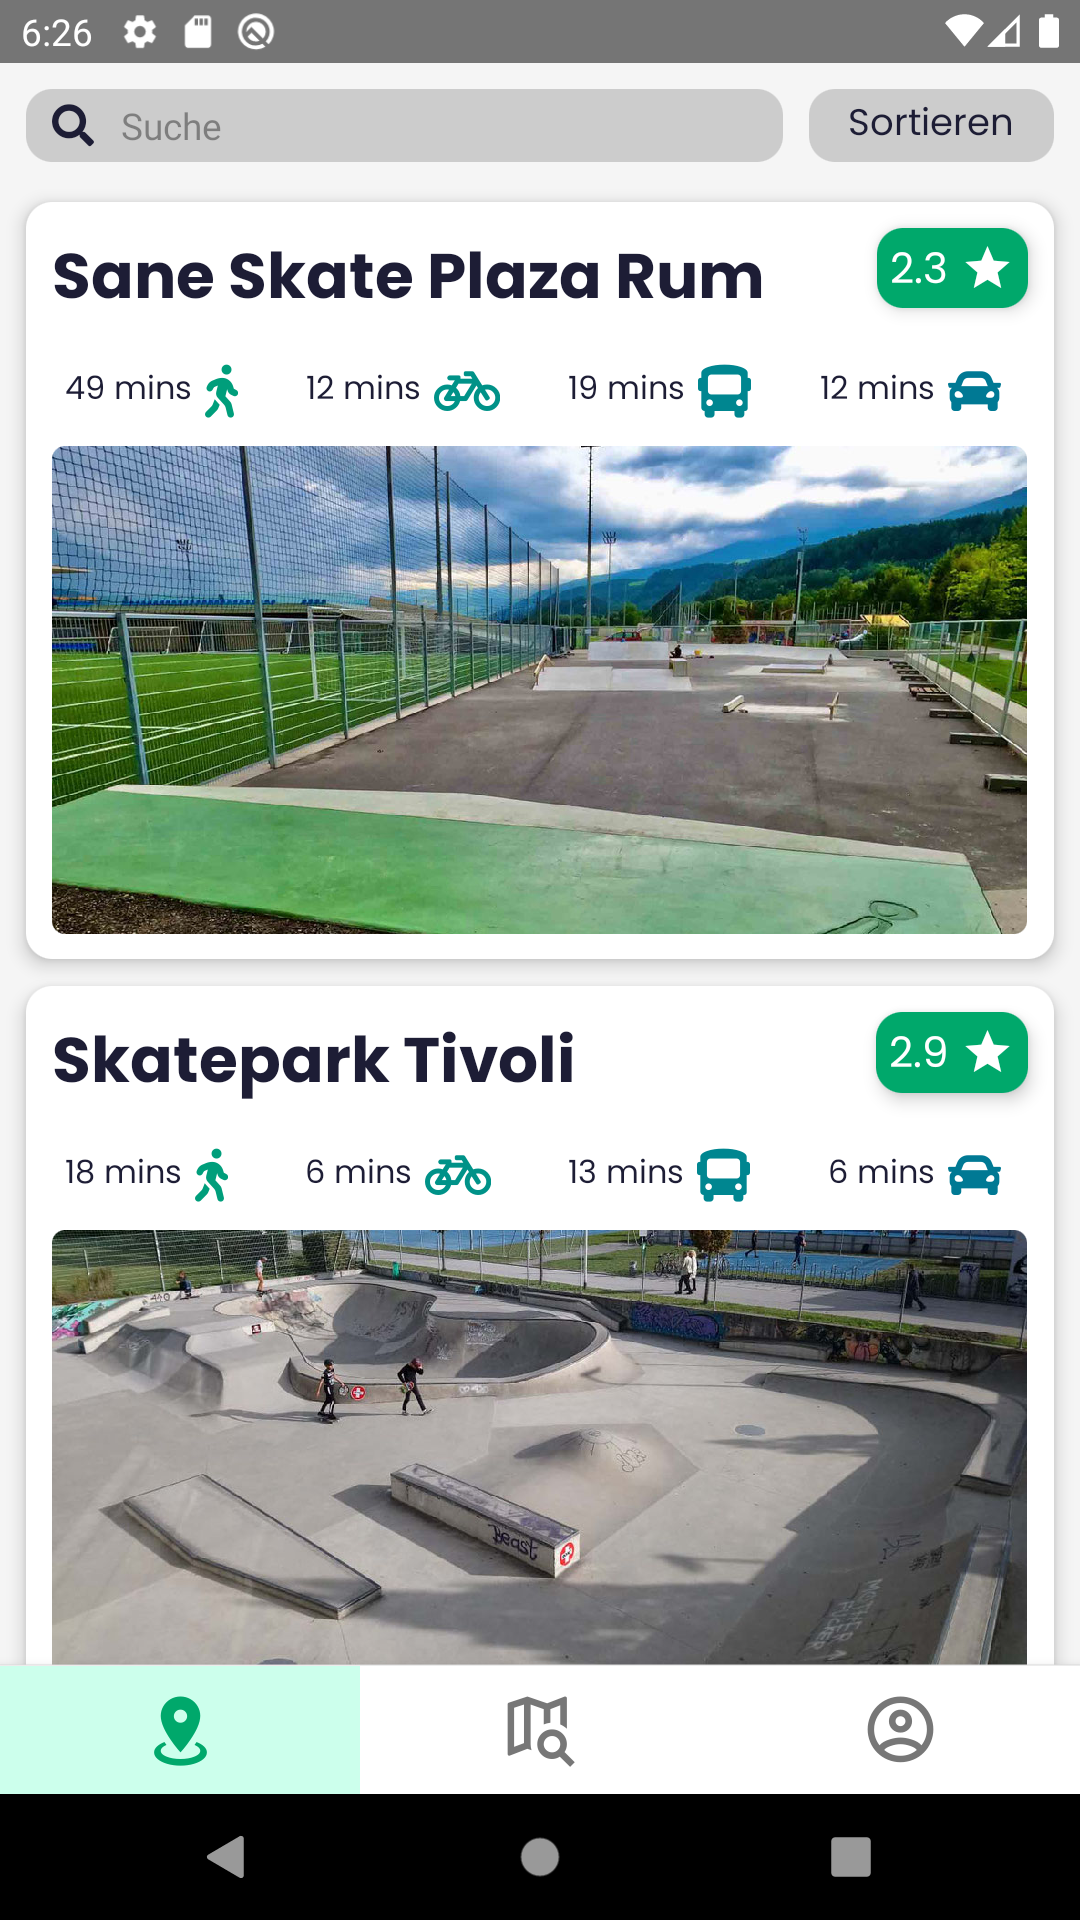
\includegraphics[width=0.6\textwidth]{Mobile/Skateparks/SkateparksList.png}
    \caption{SkateparksList Screen}
  \end{center}
\end{figure}

Wenn der Benutzer auf einen Skatepark drückt, wird bei der Navigation zu SkateparkDetails der
Skatepark übergeben, um die Informationen anzuzeigen.

Am oberen Rand des Bildschirms hat der Benutzer die Möglichkeit, nach einem bestimmten
Skateparknamen zu suchen und nach der Reisezeit zu sortieren, aufsteigend und absteigend.

\begin{figure}[H]
  \begin{center}
    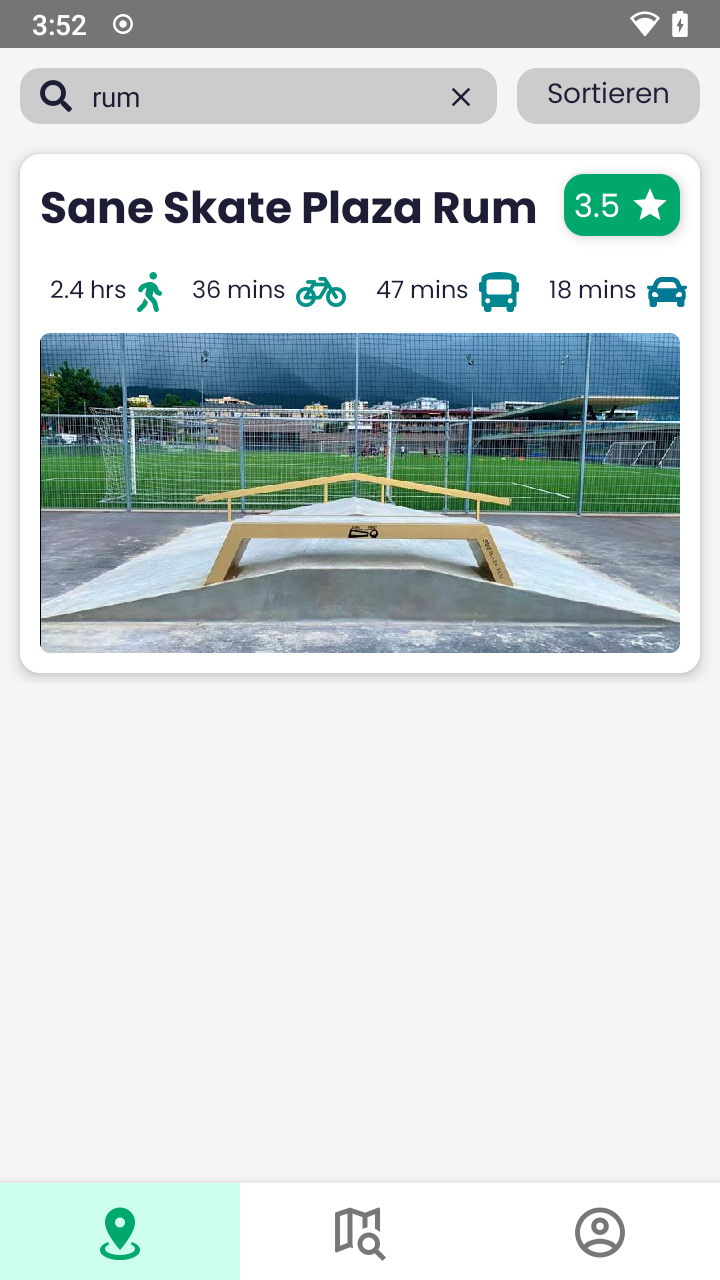
\includegraphics[width=0.6\textwidth]{Mobile/Skateparks/Search.png}
    \caption{Suchfunktion Demonstration}
  \end{center}
\end{figure}

\begin{figure}[H]
  \begin{center}
    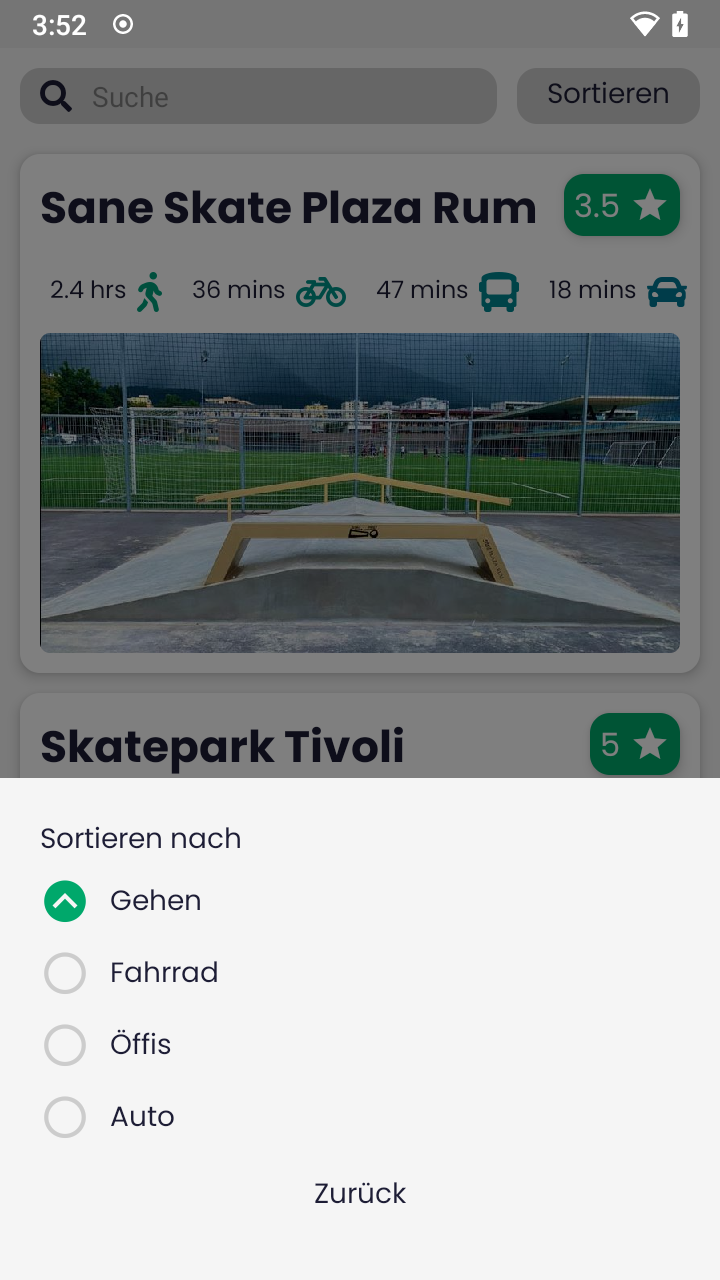
\includegraphics[width=0.6\textwidth]{Mobile/Skateparks/SortModal.png}
    \caption{Sortieren nach Zeit}
  \end{center}
\end{figure}

\newpage

\subsubsection{SkateparkDetails}
Als erstes werden die wichtigsten Informationen zum Standort des Parks angezeigt. Darunter gibt es
eine kleine Diashow mit diversen Bildern des Parks.

\begin{figure}[H]
  \begin{center}
    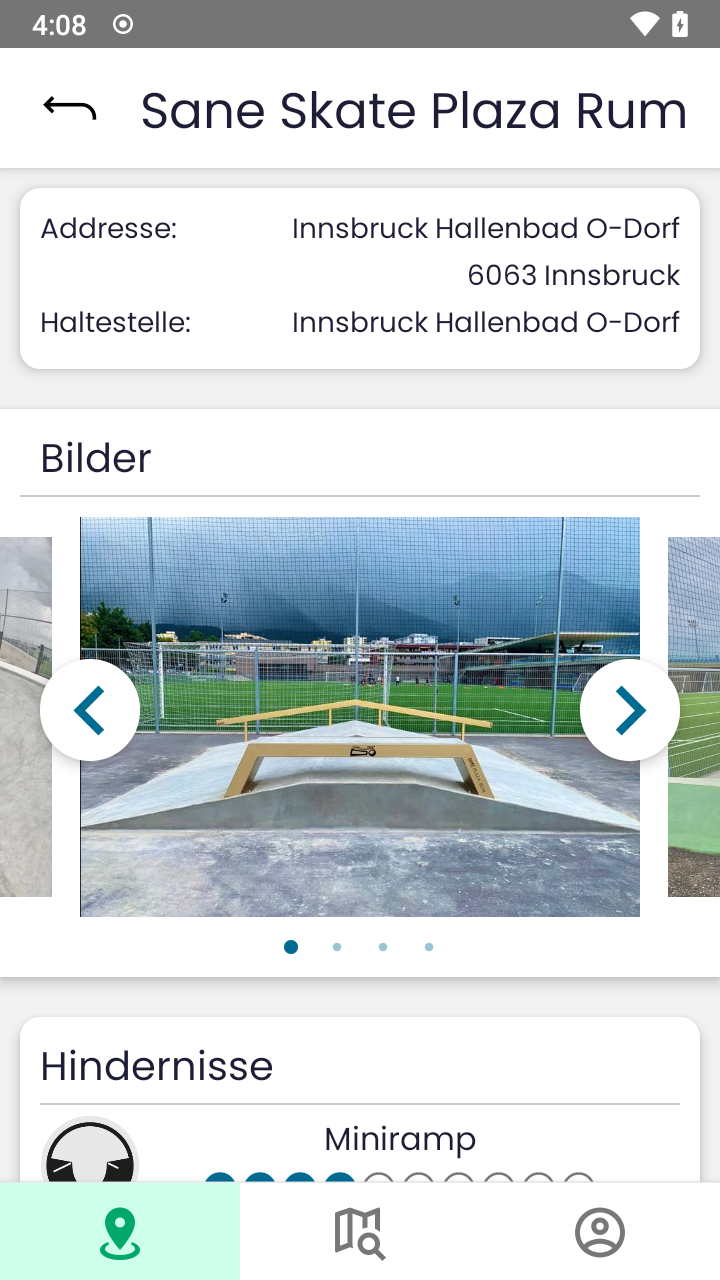
\includegraphics[width=0.6\textwidth]{Mobile/Skateparks/SkateparkDetails.png}
    \caption{Adresse und nächste Haltestelle werden als erstes gezeigt}
  \end{center}
\end{figure}

\begin{figure}[H]
  \begin{center}
    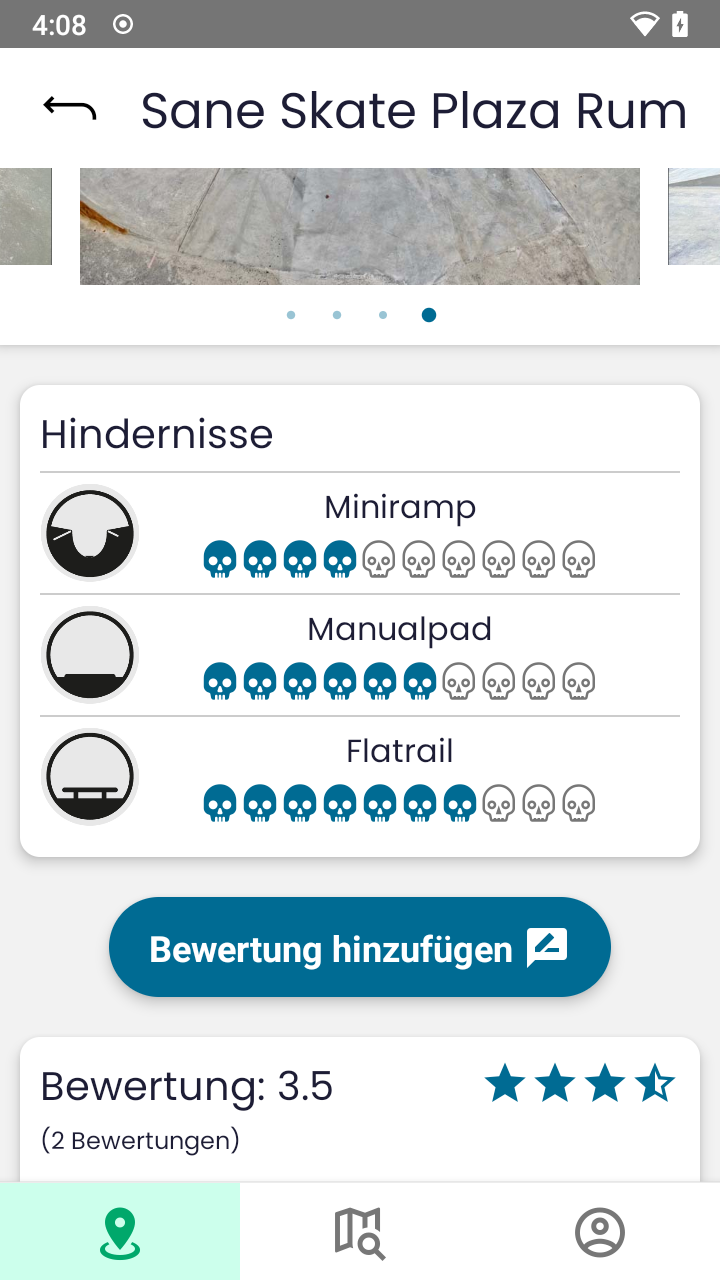
\includegraphics[width=0.6\textwidth]{Mobile/Skateparks/Obstacles.png}
    \caption{Zu jedem Park werden auch Hindernisse mit Schwierigkeitseinschätzungen abgespeichert}
  \end{center}
\end{figure}

Um eine Bewertung zu hinterlassen, drückt der Benutzer auf den Knopf "Bewertung hinzufügen" und
füllt das angezeigte Formular aus. Anschließend werden die Daten an das Backend geschickt und
abgespeichert.

\begin{figure}[H]
  \begin{center}
    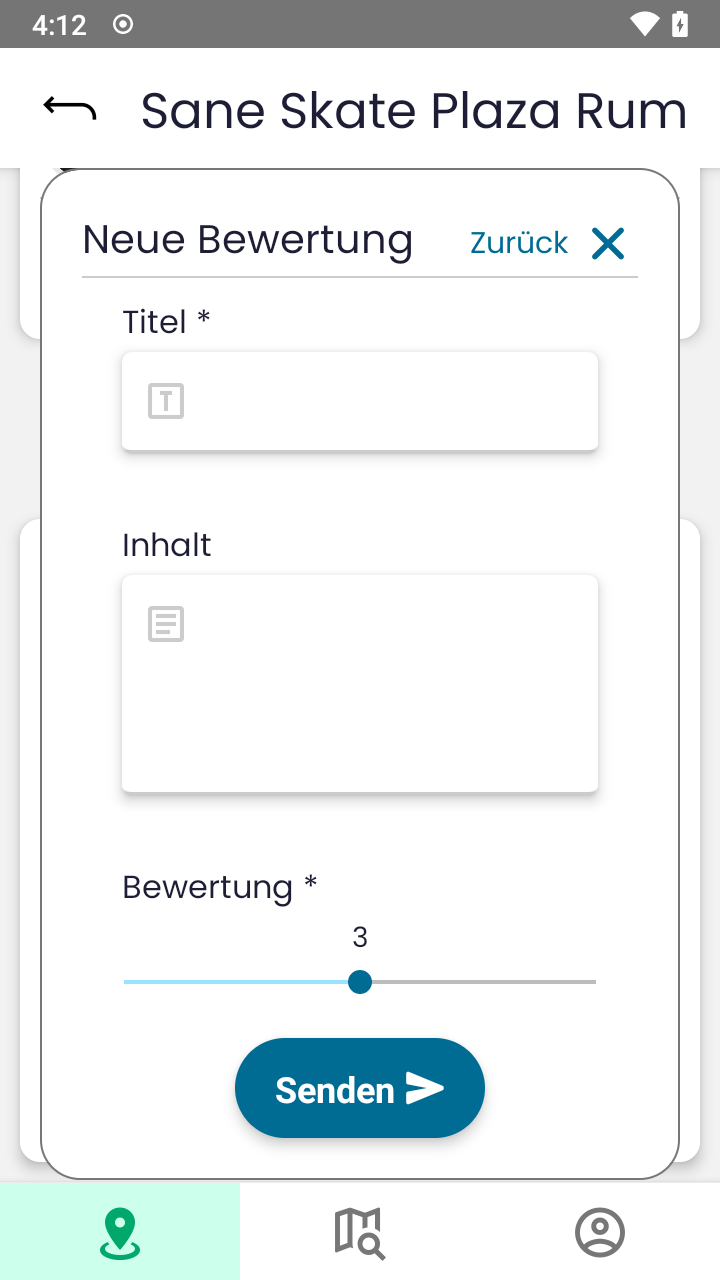
\includegraphics[width=0.6\textwidth]{Mobile/Skateparks/AddReview.png}
    \caption{Daten eintragen und absenden.}
  \end{center}
\end{figure}

Am Ende wird noch die durchschnittliche Bewertung, die Anzahl der Bewertungen und alle Bewertungen
selbst angezeigt.

\begin{figure}[H]
  \begin{center}
    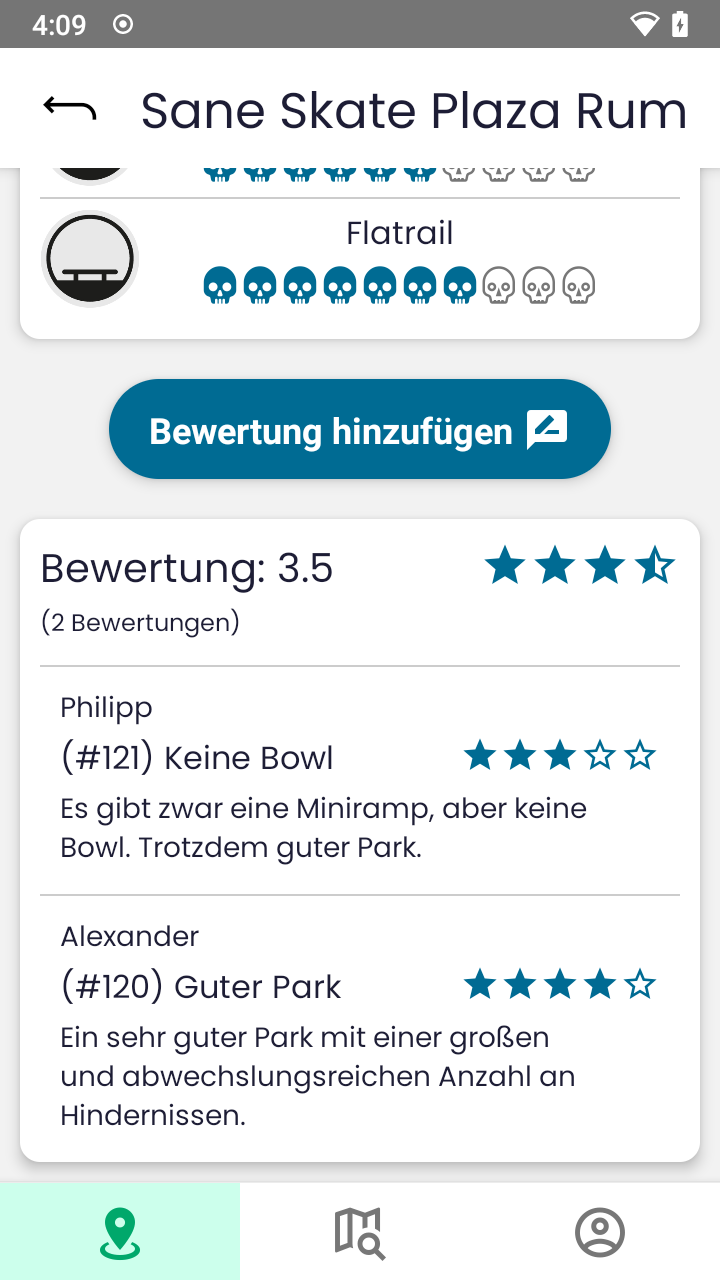
\includegraphics[width=0.6\textwidth]{Mobile/Skateparks/Reviews.png}
    \caption{Alle Bewertungen}
  \end{center}
\end{figure}

\subsection{LoginSignupStack}
Der \textbf{LoginSignupStack} besteht aus drei Screens:

\subsubsection{LoginScreen}
Im \textbf{LoginScreen} wird der Benutzer dazu aufgefordert, seine Anmeldedaten einzugeben.

\begin{figure}[H]
  \begin{center}
    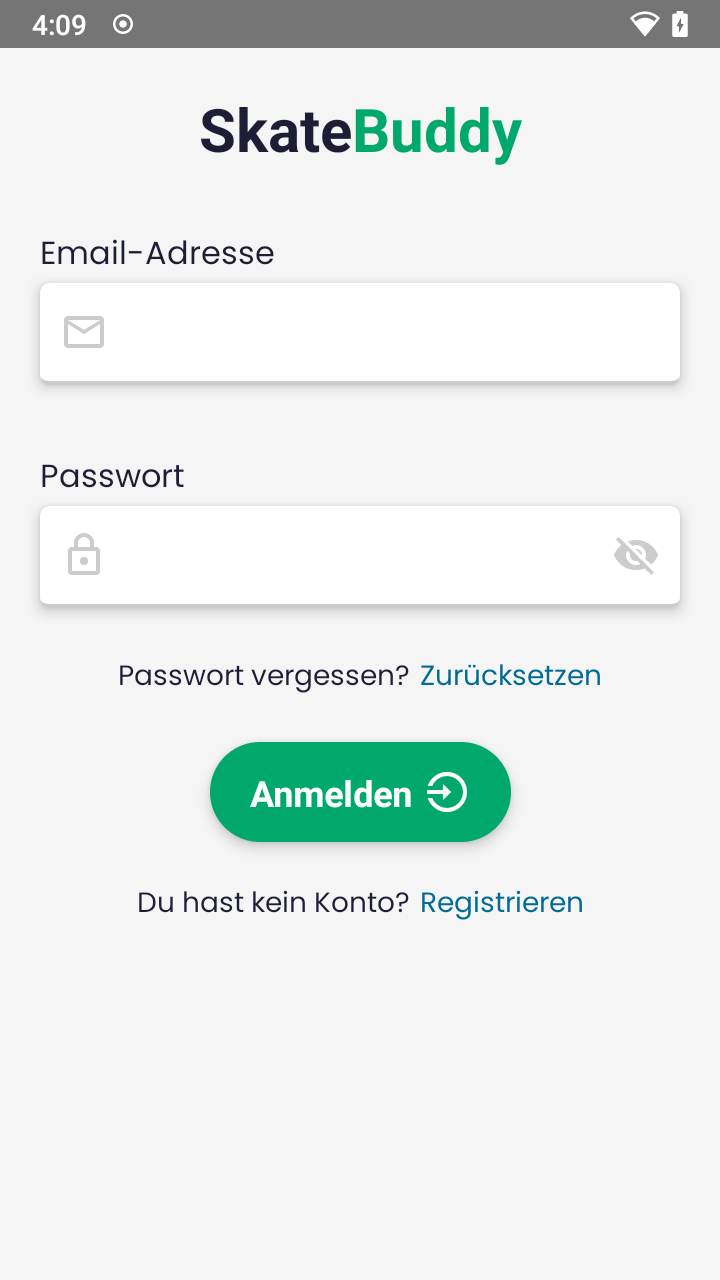
\includegraphics[width=0.6\textwidth]{Mobile/Login/Login.png}
    \caption{Daten eintragen und absenden.}
  \end{center}
\end{figure}

\subsubsection{SignupScreen}
Sollte er noch keinen Account haben, ist es ihm möglich, einen neuen Account zu erstellen über den
\textbf{SignupScreen}.

\begin{figure}[H]
  \begin{center}
    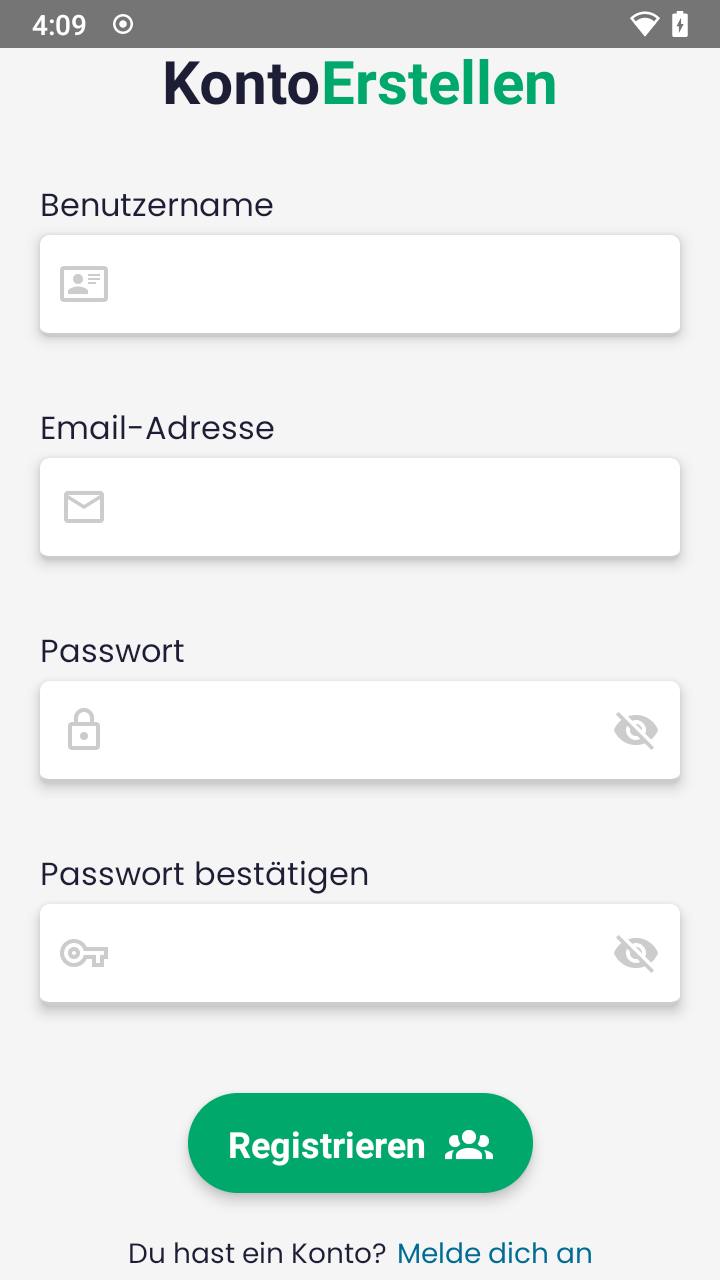
\includegraphics[width=0.6\textwidth]{Mobile/Login/Register.png}
    \caption{Daten eintragen und absenden.}
  \end{center}
\end{figure}

\subsubsection{ForgotPassword}
Wenn es dem Benutzer passieren sollte, dass er sein Passwort vergisst und keinen Zugriff auf seinen
Account mehr hat, so kann er über diesen Bildschirm einen Link anfordern, mit dem er sein Passwort
zurücksetzen kann. Dieser Link wird per E-Mail versendet.

Diese Funktion ist noch nicht in unserer App vorhanden, bis jetzt wird einfach überprüft, ob diese
E-Mail-Adresse existiert.

\begin{figure}[H]
  \begin{center}
    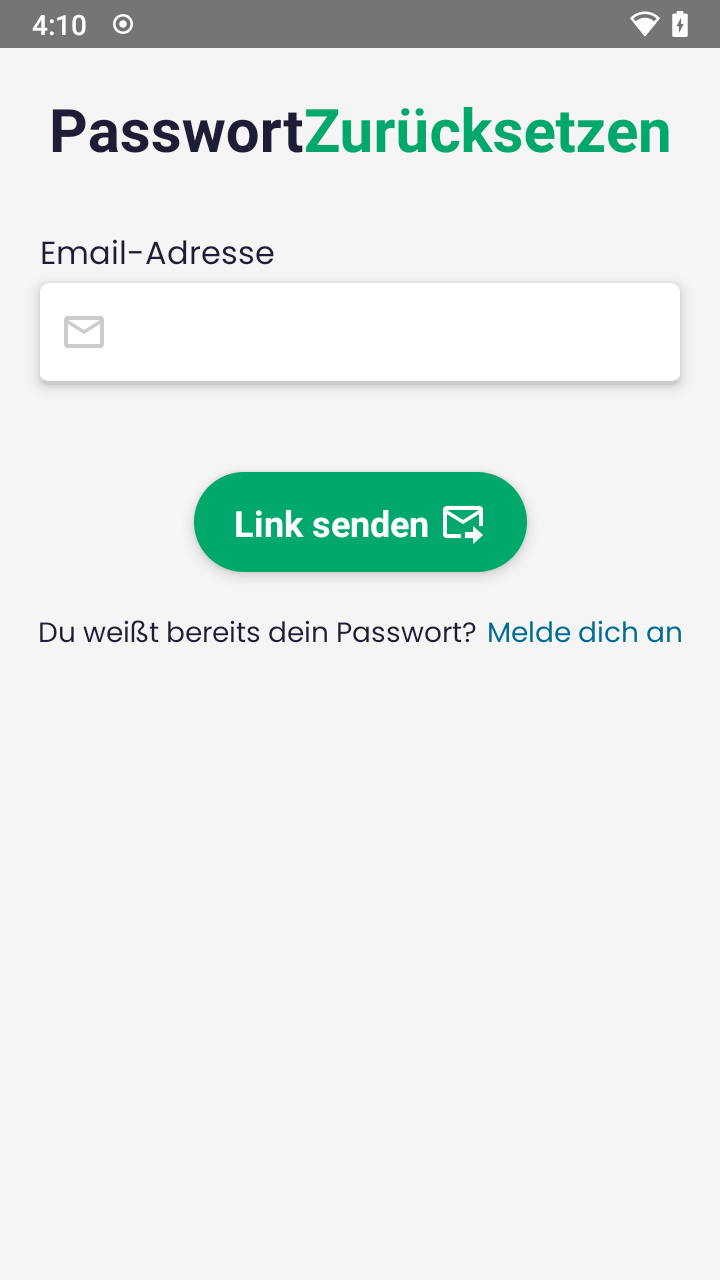
\includegraphics[width=0.6\textwidth]{Mobile/Login/Forgot.png}
    \caption{Daten eintragen und absenden.}
  \end{center}
\end{figure}


